\documentclass[letterpaper]{scrartcl}	
\usepackage[top=0.8in, bottom=1in, left=0.9in, right=0.9in]{geometry}

\makeatletter
\DeclareOldFontCommand{\tt}{\normalfont\ttfamily}{\mathtt}
\makeatother

\usepackage{url}
\usepackage{scalefnt}
\usepackage{bm}
\usepackage{cancel}

%--------------------------------------------------------------
% We need this package, part of the KOMA class, for the custom
% headings.
%--------------------------------------------------------------
\usepackage{scrpage2}	
		

%--------------------------------------------------------------
% One of many packages you can use if you want to include
% graphics.
%--------------------------------------------------------------
\usepackage{graphicx}			

%--------------------------------------------------------------
% The AMS packages are useful but not required. They offer a
% number of nice fonts, environments for formatting multiline
% equations, etc.
%--------------------------------------------------------------
\usepackage{amsmath}			
\usepackage{amsfonts}
\usepackage{amssymb}
\usepackage{amsthm}

%--------------------------------------------------------------
% Basic way to set-up the page margins.
%--------------------------------------------------------------
%\addtolength{\oddsidemargin}{-.2in}
%\addtolength{\evensidemargin}{-.2in}
%\addtolength{\textwidth}{0.45in}
%\addtolength{\topmargin}{-.175in}
%\addtolength{\textheight}{0.75in}

%--------------------------------------------------------------
% Comment out the following to add indents and remove space between paragraphs.
%--------------------------------------------------------------
\usepackage{parskip}

%--------------------------------------------------------------
% This package is used to define custom colours.
%--------------------------------------------------------------
\usepackage[usenames,dvipsnames,svgnames,table]{xcolor}

%--------------------------------------------------------------
% Package for adding in solutions:
%--------------------------------------------------------------
\usepackage[nosoln,regf,nolf]{optional}
%\usepackage[soln,regf]{optional}

%\newcommand{\soln}[1]{\opt{soln}{\\[4pt] \textcolor{JungleGreen}{\textbf{Solution:}} #1}}
\newcommand{\soln}[1]{\opt{soln}{\textcolor{JungleGreen}{\usekomafont{descriptionlabel}{Solution:}} #1}}

\newcommand{\hint}[1]{{\usekomafont{descriptionlabel}{Hint:}} #1}
\newcommand{\note}[1]{{\usekomafont{descriptionlabel}{Note:}} #1}
\newcommand{\reference}[1]{{\usekomafont{descriptionlabel}{Reference:}} #1}

%--------------------------------------------------------------
% A few colours for hyperlinks.
%--------------------------------------------------------------
\definecolor{plum}{rgb}{0.36078, 0.20784, 0.4}
\definecolor{chameleon}{rgb}{0.30588, 0.60392, 0.023529}
\definecolor{cornflower}{rgb}{0.12549, 0.29020, 0.52941}
\definecolor{scarlet}{rgb}{0.8, 0, 0}
\definecolor{brick}{rgb}{0.64314, 0, 0}

%--------------------------------------------------------------
% A command for typesetting and linking an email address.
%--------------------------------------------------------------
\newcommand{\email}[1]{\href{mailto:#1}{\tt \textcolor{cornflower}{#1}}}
\newcommand{\web}[1]{\href{#1}{\tt \textcolor{cornflower}{#1}}}

%--------------------------------------------------------------
%  The following declaration includes the hyperref package and
% assigns metadata. If you compile with pdflatex, this data
% will be automatically included in the pdf file.
%--------------------------------------------------------------
%\usepackage[
%	pdftitle={QFT Tutorial 1},%
%	pdfauthor={PSI Tutors},%
%	pdfsubject={QFT Tutorial 1},%
%	pdfkeywords={PSI},
%	colorlinks=true,
%	linkcolor=cornflower,
%	citecolor=scarlet,
%	urlcolor=chameleon%
%]{hyperref}

%\setcounter{secnumdepth}{2}	% section number depth
%\setcounter{tocdepth}{2}		% depth of TOC

%--------------------------------------------------------------
% Specify the font used in captions.
%--------------------------------------------------------------
\setkomafont{captionlabel}{\usekomafont{descriptionlabel}}

%--------------------------------------------------------------
% This is where we define the custom title. The image that is
% placed on the left-hand-side of the title, PILogo.pdf in
% this case, should be in the same directory as this file. Note
% that you can always use hyperlinks for the Title, Semester,
% and Author fields, below, in case you want to link to a seminar
% web page or a lecturer's email address.
%--------------------------------------------------------------

\titlehead{%
	\vspace*{-1cm}
	\begin{minipage}[b]{4.0cm}
	\includegraphics*[height=1.3cm]{avatar-icon.png}%
	\end{minipage}
	\hfill
	\begin{minipage}[b]{12cm}
	\begin{flushright}
		\usekomafont{descriptionlabel}
		\large Machine Learning in Condensed Matter Physics \\
		\normalsize \normalfont
		Donostia - San Sebastian, 26-28 August 2019 \hspace{1cm} Roger G. Melko
	\end{flushright}
	\end{minipage}
	\\[-3mm]
	\hrule
	\vspace{-3mm}
}
% -----------

%--------------------------------------------------------------
% Other useful physic-related packages
%--------------------------------------------------------------
\usepackage{braket}  
% Use \Bra{}, \Ket{} or \Braket{x | \psi} for Dirac notation

%--------------------------------------------------------------
% Nice numbering for question parts.
%--------------------------------------------------------------
\newcommand{\ba}{\begin{eqnarray}}
\newcommand{\ea}{\end{eqnarray}}

\newcommand{\ssk}{\smallskip}
\newcommand{\msk}{\medskip}

\newcommand{\nin}{\noindent}

\newcommand{\beq}{\begin{equation}}
\newcommand{\eeq}{\end{equation}}

\newcommand{\beqs}{\begin{equation*}}
\newcommand{\eeqs}{\end{equation*}}

\renewcommand{\vec}[1]{{\mathbf{#1}}}
\renewcommand{\labelenumi}{\alph{enumi})}
\renewcommand{\labelenumiii}{\roman{enumiii})}

%%%%%%%%%%%%%

\def\be{\begin{eqnarray}}
\def\ee{\end{eqnarray}}
\newcommand{\nn}{\nonumber}
\newcommand\para{\paragraph{}}
\newcommand{\ft}[2]{{\textstyle\frac{#1}{#2}}}
\newcommand{\eqn}[1]{(\ref{#1})}
\newcommand{\pl}[1]{\frac{\partial {\cal L}}{\partial{#1}}}
\newcommand{\ppp}[2]{\frac{\partial {#1}}{\partial {#2}}}
\newcommand{\ph}[1]{\frac{\partial {\cal H}}{\partial{#1}}}
\newcommand{\leftp}[3]{\left.\ppp{#1}{#2}\right|_{#3}}
%\newcommand{\Vec}[2]{\left(\begin{array}{c} {#1} \\ {#2}\end{array}\right)}
\newcommand\vx{\vec{x}}
\newcommand\vy{\vec{y}}
\newcommand\vp{\vec{p}}
\newcommand\vq{\vec{q}}
\newcommand\vk{\vec{k}}
\newcommand\avp{a^{\ }_{\vp}}
\newcommand\advp{a^\dagger_{\vp}}
\newcommand\ad{a^\dagger}

\newcommand\balpha{\mbox{\boldmath $\alpha$}}
\newcommand\bbeta{\mbox{\boldmath $\beta$}}
\newcommand\bgamma{\mbox{\boldmath $\gamma$}}
\newcommand\bomega{\mbox{\boldmath $\omega$}}
\newcommand\blambda{\mbox{\boldmath $\lambda$}}
\newcommand\bmu{\mbox{\boldmath $\mu$}}
\newcommand\bphi{\mbox{\boldmath $\phi$}}
\newcommand\bzeta{\mbox{\boldmath $\zeta$}}
\newcommand\bsigma{\mbox{\boldmath $\sigma$}}
\newcommand\bepsilon{\mbox{\boldmath $\epsilon$}}
\newcommand\btau{\mbox{\boldmath $\tau$}}
\newcommand\beeta{\mbox{\boldmath $\eta$}}
\newcommand\btheta{\mbox{\boldmath $\theta$}}

\def\norm#1{:\!\!#1\!\!:}

\def\part{\partial}

\def\dbox{\hbox{{$\sqcup$}\llap{$\sqcap$}}}

\def\sla#1{\hbox{{$#1$}\llap{$/$}}}
\def\Dslash{\,\,{\raise.15ex\hbox{/}\mkern-13mu D}}
\def\Dbarslash{\,\,{\raise.15ex\hbox{/}\mkern-12mu {\bar D}}}
\def\delslash{\,\,{\raise.15ex\hbox{/}\mkern-10mu \partial}}
\def\delbarslash{\,\,{\raise.15ex\hbox{/}\mkern-9mu {\bar\partial}}}
\def\pslash{\,\,{\raise.15ex\hbox{/}\mkern-11mu p}}
\def\qslash{\,\,{\raise.15ex\hbox{/}\mkern-9mu q}}
\def\kslash{\,\,{\raise.15ex\hbox{/}\mkern-11mu k}}
\def\eslash{\,\,{\raise.15ex\hbox{/}\mkern-9mu \epsilon}}
\def\calDslash{\,\,{\rais.15ex\hbox{/}\mkern-12mu {\cal D}}}
\newcommand{\slsh}[1]{\,\,{\raise.15ex\hbox{/}\mkern-12mu {#1}}}


\newcommand\Bprime{B${}^\prime$}
%\newcommand{\sign}{{\rm sign}}

\newcommand\bx{{\bf x}}
\newcommand\br{{\bf r}}
\newcommand\bF{{\bf F}}
\newcommand\bp{{\bf p}}
\newcommand\bL{{\bf L}}
\newcommand\bR{{\bf R}}
\newcommand\bP{{\bf P}}
\newcommand\bE{{\bf E}}
\newcommand\bB{{\bf B}}
\newcommand\bA{{\bf A}}
\newcommand\bee{{\bf e}}
\newcommand\bte{\tilde{\bf e}}
\def\ket#1{\left| #1 \right\rangle}
\def\bra#1{\left\langle #1 \right|}
\def\vev#1{\left\langle #1 \right\rangle}

\newcommand\lmn[2]{\Lambda^{#1}_{\ #2}}
\newcommand\mup[2]{\eta^{#1 #2}}
\newcommand\mdown[2]{\eta_{#1 #2}}
\newcommand\deld[2]{\delta^{#1}_{#2}}
\newcommand\df{\Delta_F}
\newcommand\cL{{\cal L}}
%\def\theequation{\thesection.\arabic{equation}

\newcounter{solneqn}
%\newcommand{\mytag}{\refstepcounter{equation}\tag{\roman{equationn}}}
\newcommand{\mytag}{\refstepcounter{solneqn}\tag{S.\arabic{solneqn}}}
%%%%%%%%%


\DeclareMathOperator{\Tr}{Tr}
\DeclareMathOperator{\sign}{sign}

%\renewcommand{\ttdefault}{pcr}

\usepackage{enumitem}

\begin{document}

%\scalefont{1.35}

\vspace{-3cm}

\opt{nosoln}{\title{Tutorial: \\Learning classical thermodynamic observables with \\restricted Boltzmann machines \vspace*{-6mm}}}
\opt{soln}{\title{Tutorial \textcolor{JungleGreen}{Solutions}: \\Learning classical thermodynamic observables with \\restricted Boltzmann machines \vspace*{-6mm}}}

\date{August 30, 2019}

\maketitle

The objective of this tutorial is to train a restricted Boltzmann machine (RBM) on spin configurations 
and then sample new spin configurations from the trained RBM. 
You will compute thermodynamic observables from these samples and compare to known results (from Monte Carlo simulation).
You will use and modify the Python programs 
\texttt{rbm.py}, \texttt{tutorial4{\textunderscore}train{\textunderscore}ising2d.py} and 
\texttt{tutorial4{\textunderscore}sample{\textunderscore}ising2d.py} %and \texttt{tutorial5{\textunderscore}plot{\textunderscore}results.py}.

As seen in the lectures, the architecture of a RBM can be represented as
\begin{center}
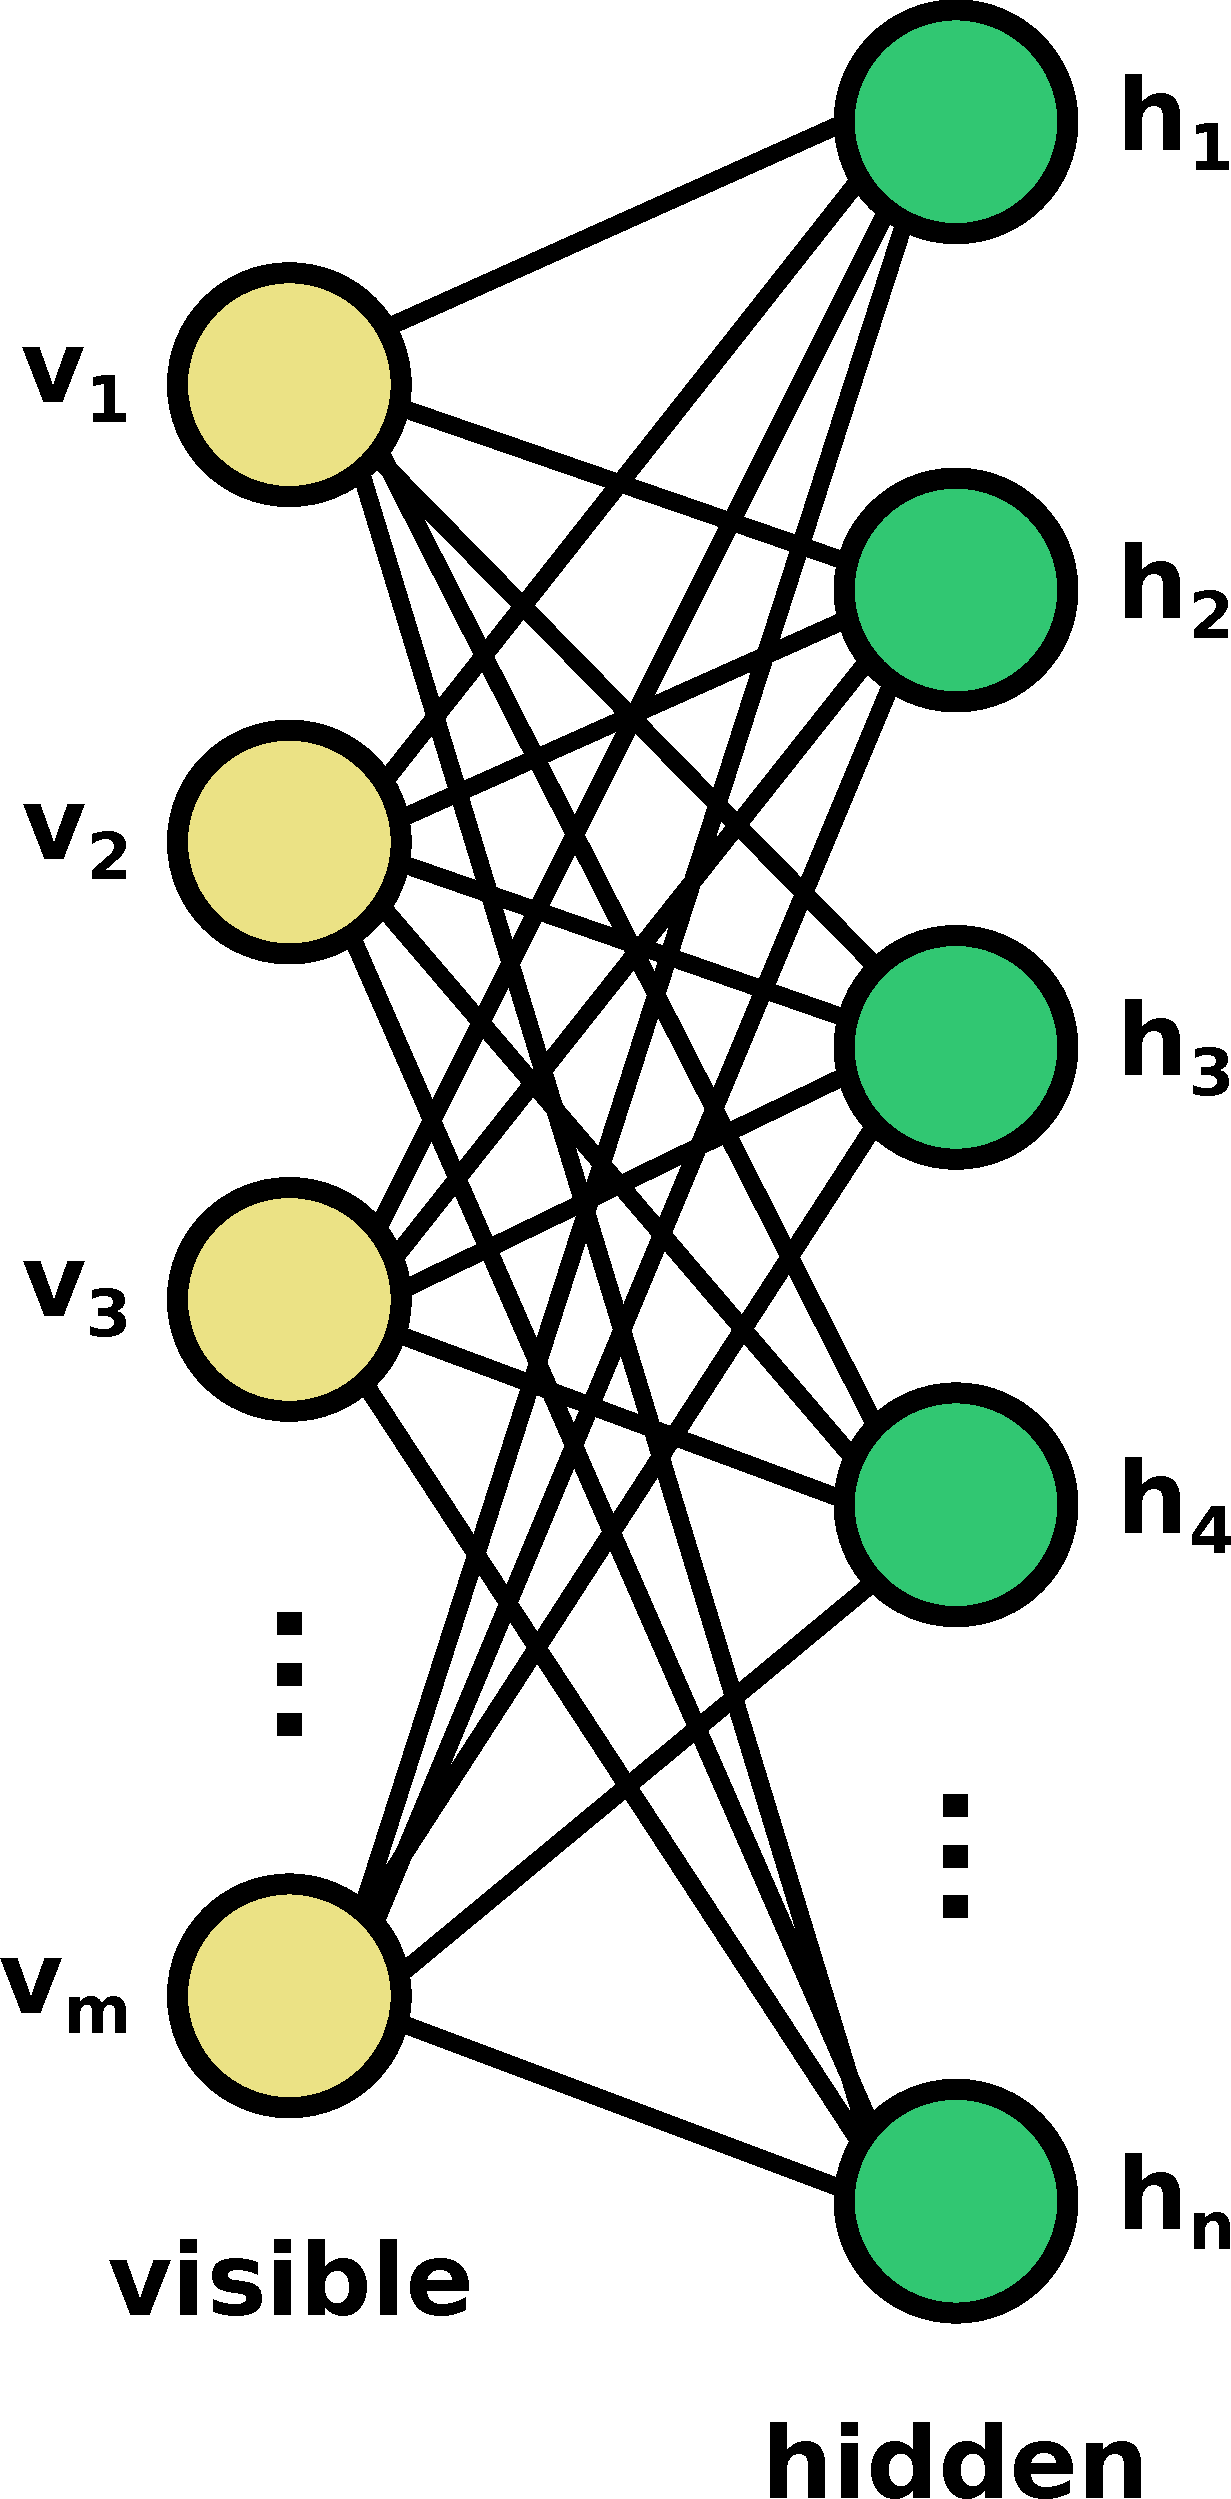
\includegraphics[width=4cm]{RBM.pdf}
\end{center}
where $\mathbf{v} = \left(v_1, v_2, \ldots v_m\right)^T$ consists of $m$ visible units with $v_i \in \{0,1\}$ and $\mathbf{h} = \left(h_1, h_2, \ldots h_n\right)^T$ consists of $n$ hidden units with $h_j \in \{0,1\}$.
The weights of the RBM are denoted as $W_{ij}$. 
The biases are denoted as $b_i$ for the visible units and $c_j$ for the hidden units.
We use $\lambda$ to denote all model parameters such that $\lambda = \{ W, b, c \}$.
Within the given python programs, the number of visible units $m$ is stored in the variable \texttt{num{\textunderscore}visible}
and the number of hidden units $n$ is stored in the variable \texttt{num{\textunderscore}hidden}.

The probability distribution associated with the RBM is given by
\begin{equation*}
p_\lambda(\mathbf{v}, \mathbf{h}) = \frac{1}{Z_\lambda} e^{-E_\lambda (\mathbf{v}, \mathbf{h})},
\end{equation*}
where
\begin{equation*}
E_\lambda (\mathbf{v}, \mathbf{h}) = -\sum_{i=1}^m b_i \, v_i -\sum_{j=1}^n c_j\,  h_j - \sum_{ij} W_{ij} \, v_i \, h_j ,
\end{equation*}
and 
\begin{equation*}
Z_\lambda = \sum_{\mathbf{v}, \mathbf{h}} e^{-E_\lambda (\mathbf{v}, \mathbf{h})}.
\end{equation*}

You will train an RBM to learn the distribution corresponding to spin configurations of 
the two-dimensional classical Ising model on an $L=4$ lattice at a given temperature.
The number of visible units will be equal to the number of spins $N$ such that $m = N = L^2 = 16$.
You have been given data corresponding to 11 different temperatures (1.0, 1.254, 1.508, 1.762, 2.016, 2.269, 2.524, 2.778, 3.032, 3.286 and 3.54) in the folder \texttt{MC{\textunderscore}results}.
We know that these configurations are generated (using Monte Carlo simulation) according to the Boltzmann distribution
\beq
q(\mathbf{v},T) = \frac{1}{Z} e^{-H(\mathbf{v})/T}, 
\eeq
where $Z = \sum_{\{ \mathbf{v} \}}e^{-H(\mathbf{v})/T}$ is the partition function and $H(\mathbf{v}) = -J \sum_{\langle i j \rangle} v_i v_j$ is the Ising model Hamiltonian with critical temperature $T_\text{c} \approx 2.269 J$.
We wish to adjust the RBM parameters $\lambda$ such that the RBM distribution $p_\lambda(\mathbf{v})$ is a good approximation of $q(\mathbf{v},T)$.
This training is done by minimizing the negative log-likelihood (NLL), which is equivalent to minimizing the Kullback-Liebler (KL) divergence. 
The RBM never has explicit knowledge of $q(\mathbf{v},T)$ or $H(\mathbf{v})$.

After training the RBM, we can then sample from it new spin configurations.
Based on our theoretical knowledge of the Ising model, we can compute observables such as 
the energy $E(\mathbf{v})$, magnetization $M(\mathbf{v})$, specific heat $C_v(\mathbf{v})$ and susceptibility $\chi(\mathbf{v})$ for each sample.
Assuming units where $J = k_\text{B} = 1$, we have
\begin{align*}
E(\mathbf{v}) &= H(\mathbf{v}) = -\sum_{\langle i j \rangle} v_i v_j, \\
M(\mathbf{v}) &= \sum_i v_i , \\
C_v(\mathbf{v}) &= \frac{\langle E^2 \rangle - \langle E \rangle^2}{T^2}, \\
\chi(\mathbf{v}) &= \frac{\langle M^2 \rangle - \langle M \rangle^2}{T}.
\end{align*}
When calculating these observables for a given spin configuration $\mathbf{v} = (v_1, v_2, \ldots, v_N)$, we note that the underlying lattice has periodic boundary conditions and uses a labelling for the sites such that, for example, on a $3\times 3$ lattice:
\begin{center}
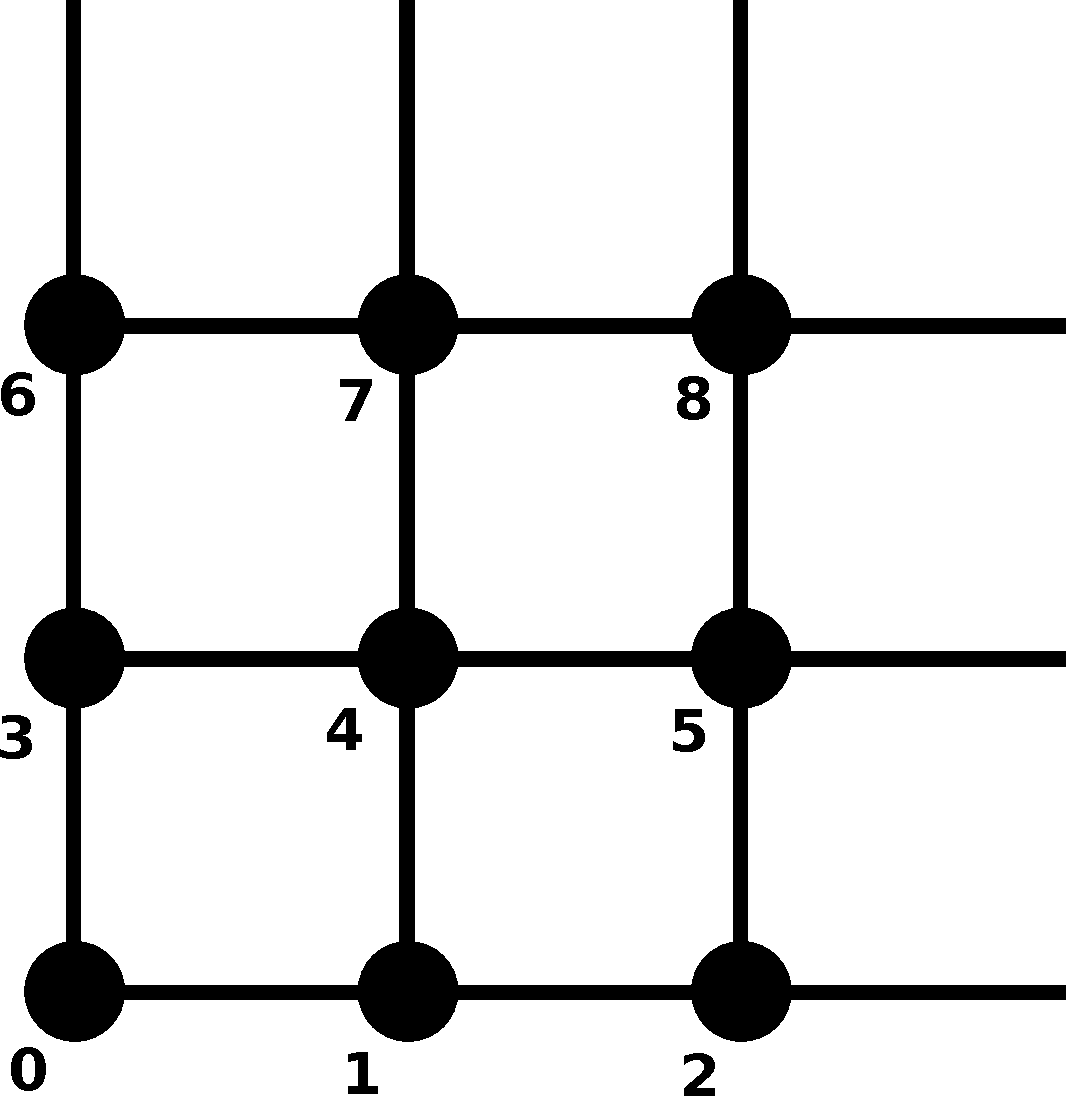
\includegraphics[width=5cm]{lattice.pdf}
\end{center}
We will compare the averages of our RBM-sampled observables to the known values we expect to find in Monte Carlo simulation.
We will also explore how the number of hidden units $n$ affects this comparison.

%In this tutorial, you will work in groups of 3--4 to answer the following questions.

%\opt{soln}{\newpage}
\begin{enumerate}[label=\alph*)]

%%%%%%%%%%%%%% (a) %%%%%%%%%%%%%%
\item Start by examining Figure 4 of Reference~\cite{giac}. How do the thermodynamic observables generated from the RBM depend on the number of hidden units $n = n_h$? How does the accuracy of each observables vary with the distance from the critical temperature $T_\text{c}$? 

%%% SOLUTION %%%
\soln{
}

%%%%%%%%%%%%%% (b) %%%%%%%%%%%%%%
\item Let us train our first RBM at the critical temperature $T_\text{c}$ with $n=4$ hidden units. 
Run the code \texttt{tutorial4{\textunderscore}train{\textunderscore}ising2d.py} with \texttt{T = 2.269} and \texttt{num{\textunderscore}hidden = 4}.
This code will train the parameters $\lambda$ of an RBM based on the given Monte Carlo samples such that 
$p_\lambda(\mathbf{v})$ is a good approximation of $q(\mathbf{v},T)$.
The resulting parameters will be saved to a file within the folder \texttt{RBM{\textunderscore}parameters}.
Increase the parameter \texttt{nsteps} until you are convinced that the NLL has roughly converged.
%\item For each of the 11 temperatures, run the code \texttt{tutorial5{\textunderscore}train{\textunderscore}ising2d.py}.
%For each temperature $T$, this code will train the parameters $\lambda$ of an RBM based on the Monte Carlo samples such that 
%$p_\lambda(\mathbf{v})$ is a good approximation of $q(\mathbf{v},T)$.

%\hint{Since some temperatures might take longer to train, you may wish to have each group member study different temperatures.}

%%% SOLUTION %%%
\soln{
}

%%%%%%%%%%%%%% (c) %%%%%%%%%%%%%%
\item Examine the parameters \texttt{learning{\textunderscore}rate{\textunderscore}start}, \texttt{bsize}, \texttt{num{\textunderscore}gibbs} and  \texttt{num{\textunderscore}samples} and explain how each are used to train the RBM.
Experiment with adjusting each of these parameters to see how it affects the training behaviour.

%%% SOLUTION %%%
\soln{
}

%%%%%%%%%%%%%% (d) %%%%%%%%%%%%%%
\item Run \texttt{tutorial4{\textunderscore}sample{\textunderscore}ising2d.py} (again with with \texttt{T = 2.269} and \texttt{num{\textunderscore}hidden = 4}) to generate new spin configuration samples.
This program will also save the sample configurations to a file within the folder \texttt{RBM{\textunderscore}samples}.
%This program will also save the corresponding average energy, magnetization, specific heat and susceptibility for each temperature
%in a file within the folder \texttt{RBM{\textunderscore}observables}.

%%% SOLUTION %%%
\soln{
}

\begin{table*}[t]
\begin{center}
\begin{tabular}{ | c | c | c | c | c |  }
\hline
 $T$ & $\langle E \rangle /N $ & $\langle M \rangle /N $ & $C_v /N $ & $\chi /N $  \\ 
\hline%{|=|==|====|}
1.508 & -1.9451(9)  & 0.9856(2)  & 0.25(2)  & 0.030(4)  \\  
2.269 &  -1.514(2) & 0.849(1) & 1.06(2)  & 0.316(9)  \\  
3.286  & -0.744(2)  & 0.532(1) & 0.574(6)  & 0.408(6)  \\  
%\hhline{|=|==|====|}
\hline

\hline
\end{tabular}
\end{center}
	\caption{ 
	Thermodynamic observables measured on the Monte Carlo configurations used to train an RBM at various temperatures. Errors are indicated in parentheses. }
	\label{tab}
\end{table*}

%%%%%%%%%%%%%% (e) %%%%%%%%%%%%%%
%\item Run \texttt{tutorial5{\textunderscore}plot{\textunderscore}results.py} plot your samples' expectation values 
%and compare with known results from Monte Carlo.
\item Write code that reads in the sampled configurations generated in part d) and calculates the corresponding observables $\langle E \rangle /N $, $\langle M \rangle /N $, $C_v /N $ and $\chi /N $.
Compare with the results for the training samples, which are provided in Table~\ref{tab}.
Are your discrepancies similar to those found in Figure 4 of Reference~\cite{giac}?

\hint{In order to check if your code is working, you can try calculating the observable quantities for the training configurations in the folder \texttt{MC{\textunderscore}results} and verifying that you get the same results as in Table~\ref{tab}.}

%%%%%%%%%%%%%% (f) %%%%%%%%%%%%%%
\item Repeat parts b), d) and e) for other values of the number of hidden units $n$.
Once again consider how your results compare with Figure 4 of Reference~\cite{giac}.

%%%%%%%%%%%%%% (g) %%%%%%%%%%%%%%
\item Repeat parts b), d), e) and f) for temperatures above and below the critical temperature, such as the ones provided in Table~\ref{tab}.
How does the difference between your sampled and trained observables depend on temperature?
Once again examine how your results compare with Figure 4 of Reference~\cite{giac}.

%%% SOLUTION %%%
\soln{
}


\end{enumerate}

\begin{thebibliography}{}

\bibitem{giac} 
G. Torlai and R. Melko, Phys. Rev. B \textbf{94}, 165134 (2016), {\small\url{https://arxiv.org/abs/1606.02718}}.

\end{thebibliography}

\end{document}